%%%%%%%%%%%%%%%%%%%%%%%%%%%%%%%%%%%%%%%%%%%%%%%%%%%%%%%%%%%%%%%%%%%%%%%%%%%%%
%%%%%%                                                                  %%%%% 
%%%%%%          Maqueta de memòria TFC/PFC de l'EETAC                   %%%%% 
%%%%%%                                                                  %%%%% 
%%%%%%%%%%%%%%%%%%%%%%%%%%%%%%%%%%%%%%%%%%%%%%%%%%%%%%%%%%%%%%%%%%%%%%%%%%%%%
%%%%%%%%%%%%%%%%%%%%%%%%%%%%%%%%%%%%%%%%%%%%%%%%%%%%%%%%%%%%%%%%%%%%%%%%%%%%%
%%                                                                         %%
%%          Autor: Xavier Prats i Menéndez (xavier.prats@upc.edu)          %% 
%%                  Technical University of Catalonia (UPC)                %%
%%                                                                         %%
%%%%%%%%%%%%%%%%%%%%%%%%%%%%%%%%%%%%%%%%%%%%%%%%%%%%%%%%%%%%%%%%%%%%%%%%%%%%%
%%      This work is licensed under the Creative Commons  Attribution-     %%
%%   -Noncommercial-Share Alike 3.0 Spain License. To view a copy of this  %% 
%%    license, visit http://creativecommons.org/licenses/by-nc-sa/3.0/es/  %%
%%    or send a letter to Creative Commons, 171 Second Street, Suite 300,  %%
%%                  San Francisco,California, 94105, USA.                  %%
%%%%%%%%%%%%%%%%%%%%%%%%%%%%%%%%%%%%%%%%%%%%%%%%%%%%%%%%%%%%%%%%%%%%%%%%%%%%%
%% Versió 2.1 - Juliol 2012                                                %%
%%%%%%%%%%%%%%%%%%%%%%%%%%%%%%%%%%%%%%%%%%%%%%%%%%%%%%%%%%%%%%%%%%%%%%%%%%%%%

%%% NOTA: els seguents packages son necessaris per utilitzar la
%%%       plantilla seguent:
%%%       ifthen,calc,helvet,pslatex,fancyhdr,nextpage,subfigure,tocloft,graphicx,url

%%% NOTA: Es possible que algunes distribuicions Linux o Windows.
%%%       no portin aquests paquets instal·lats per defecte.
%%%       En aquest cas els haureu d'instal·lar manualment.


%%%%%%%%%%%%%%%%%%%%%%%%%%%%%%%%%%%%%%%%%%%%%%%%%%%%%%%%%%%%%%%%%%%%%%%%%%%%%
% 1- INICIALITZACIÓ
%%%%%%%%%%%%%%%%%%%%%%%%%%%%%%%%%%%%%%%%%%%%%%%%%%%%%%%%%%%%%%%%%%%%%%%%%%%%%

\documentclass[catalan,final]{setup/eetac_tfc_pfc}
%% * OPCIONS A CONFIGURAR al \documentclass
%%    - Estat del document: final o draft
%%      NOTA: Draft no inserta les figures i marca només l'espai que
%%      ocupen. També s'indica quan el text sobrepassa els marges.
%%      Draft és molt útil per compilar ràpid el document si no és important
%%      en aquell moment visualitzar les figures.
%%    - Idioma PRINCIPAL del document: catalan, spanish, english, french...

\usepackage[english,catalan]{babel}
%%  * INCLOURE TOTS ELS IDIOMES QUE S'USARAN EN EL DOCUMENT
%%    NOTA: per canviar d'idioma al mig del document usar:
%%          \selectlanguage{nom_idioma}
%%%%%%%%%%%%%%%%%%%%%%%%%%%%%%%%%%%%%%%%%%%%%%%%%%%%%%%%%%%%%%%%%%%%%%%%%%%%%

%%%%%%%%%%%%%%%%%%%%%%%%%%%%%%%%%%%%%%%%%%%%%%%%%%%%%%%%%%%%%%%%%%%%%%%%%%%%%
% 2- CÀRREGA DE PAQUETS ADICIONALS (OPCIONALS)
%%%%%%%%%%%%%%%%%%%%%%%%%%%%%%%%%%%%%%%%%%%%%%%%%%%%%%%%%%%%%%%%%%%%%%%%%%%%%

%%% NOTA: Es possible que algunes distribuicions Linux o Windows.
%%%       no portin aquests paquets instal·lats per defecte.
%%%       En aquest cas els haureu d'instal·lar manualment.

%% El paquet inputenc és extramadament útil. 
%% Permet escriure els accents directament amb l'editor de texte
%% sense haver de fer coses com per exemple: introducci\'o
%% Heu d'especificar la codificació de caracters que utilitzeu pel
%% vostre fitxer (en aquest exemple utf8)
\usepackage[utf8]{inputenc}

%% Símbols matemàtics de la American Mathematical Society
\usepackage{amssymb,amsmath, amsfonts}  

%% El paquet array proporciona eines molt útils a l'hora de fer 
%% equacions amb matrius
\usepackage{array}             

%% Paquet que permet fer taules fusionant cel·les de files consecutives
\usepackage{multirow}          

%% Paquet molt útil en cas de tenir taules molt llargues que 
%   ocupin vàries pàgines
\usepackage{longtable}          

%% Permet canviar els colors del document
%\usepackage{color,colortbl}

%% Paquet molt útil que permet activar links en el PDF final.
%% * NO OBLIDAR DE CONFIGURAR els quatre primer camps!
\usepackage[
  pdfauthor={Nom Cognoms autor},            % Configurar adientment
  %pdftitle={Treball Fi de Carrera - autor}, % Configurar adientment
  %pdfsubject={Titol del TFC aqui},          % Configurar adientment
  % Modificació respecte a la versió 2.1 - Iván Padilla Montero - Juliol 2014
  pdftitle={Treball Fi de Grau - autor}, % Configurar adientment
  pdfsubject={Titol del TFG aqui},          % Configurar adientment  
  pdfkeywords={keyword1, keyword2, ...},    % Configurar adientment
  pdfcreator={EETAC-UPC}, 
  pdfproducer={LaTeX, dvipdf},
  pdfdisplaydoctitle=true, plainpages=false, linktocpage=true,         
  colorlinks=true, linkcolor=blue,citecolor=blue,urlcolor=blue,
  hyperfootnotes=false, pagebackref=true, pdfpagelabels=true,
  pdfpagemode=UseOutlines,
]{hyperref} 

%% NOTA IMPORTANT!:
%% Per tal que hyperef funcioni correctament amb els capitols o seccions no
%% numerats (\chapter*{}), com per exemple introducció, conclusions i bibliografia
%% cal posar les dues comandes seguents ABANS del \chapter*{} en questió
%\cleardoublepage
%\phantomsection

%% Permet trencar links URL. 
%% Atenció! afegir aquest paquet DESPRES del hyperref!!
\usepackage{breakurl} 

%% Permet arranjar matricialment multiples figures
%% NOTA: afegir aquest paquet DESPRES del hyperref!!
%%       Si no es desitja utilitzar aquest paquet, comentar la linia seguent
%%       i anar TAMBE al fitxer de classe (eetac_tfc_pfc.cls) per substituir: 
%%       \RequirePackage[subfigure]{tocloft}  per  \RequirePackage{tocloft}
\usepackage{subfigmat}         

%%%%%%%%%%%%%%%%%%%%%%%%%%%%%%%%%%%%%%%%%%%%%%%%%%%%%%%%%%%%%%%%%%%%%%%%%%%%%


%%%%%%%%%%%%%%%%%%%%%%%%%%%%%%%%%%%%%%%%%%%%%%%%%%%%%%%%%%%%%%%%%%%%%%%%%%%%%
% 3- DOCUMENT
%%%%%%%%%%%%%%%%%%%%%%%%%%%%%%%%%%%%%%%%%%%%%%%%%%%%%%%%%%%%%%%%%%%%%%%%%%%%%

%%% Configuració de les dades i variables boleanes rellevants del document:
%%%%%%%%%%%%%%%%%%%%%%%%%%%%%%%%%%%%%%%%%%%%%%%%%%%%%%%%%%%%%%%%%%%%%%%%%%%%%
%%%%%%                                                                  %%%%% 
%%%%%%       Fitxer de dades per la memoria TFC/PFC de l'EETAC          %%%%% 
%%%%%%                                                                  %%%%% 
%%%%%%%%%%%%%%%%%%%%%%%%%%%%%%%%%%%%%%%%%%%%%%%%%%%%%%%%%%%%%%%%%%%%%%%%%%%%%
%%%%%%%%%%%%%%%%%%%%%%%%%%%%%%%%%%%%%%%%%%%%%%%%%%%%%%%%%%%%%%%%%%%%%%%%%%%%%
%%                                                                         %%
%%          Autor: Xavier Prats i Menendez (xavier.prats@upc.edu)          %% 
%%                  Technical University of Catalonia (UPC)                %%
%%                                                                         %%
%%%%%%%%%%%%%%%%%%%%%%%%%%%%%%%%%%%%%%%%%%%%%%%%%%%%%%%%%%%%%%%%%%%%%%%%%%%%%
%%      This work is licensed under the Creative Commons  Attribution-     %%
%%   -Noncommercial-Share Alike 3.0 Spain License. To view a copy of this  %% 
%%    license, visit http://creativecommons.org/licenses/by-nc-sa/3.0/es/  %%
%%    or send a letter to Creative Commons, 171 Second Street, Suite 300,  %%
%%                  San Francisco,California, 94105, USA.                  %%
%%%%%%%%%%%%%%%%%%%%%%%%%%%%%%%%%%%%%%%%%%%%%%%%%%%%%%%%%%%%%%%%%%%%%%%%%%%%%
%% Versio 2.1 - Juliol 2012                                                %%
%%%%%%%%%%%%%%%%%%%%%%%%%%%%%%%%%%%%%%%%%%%%%%%%%%%%%%%%%%%%%%%%%%%%%%%%%%%%%

%%%%%%%%%%%%%%%%%%%%%%%%%%%%%%%%%%%%%%%%%%%%%%%%%%%%%%%%%%%%%%%%%%%%%%%%%%%%%%%
%%  VARIABLES A CONFIGURAR                                                  %%%
%%%%%%%%%%%%%%%%%%%%%%%%%%%%%%%%%%%%%%%%%%%%%%%%%%%%%%%%%%%%%%%%%%%%%%%%%%%%%%%

%% - Projecte o Treball de Fi de Carrera?
%%      PFC = true   -> Projecte de Fi de Carrera
%%      PFC = false  -> Treball  de Fi de Carrera
\setboolean{PFC}{false}

%% - Escollir la titulació
%\titulacio{Enginyeria Tècnica Aeronàutica, especialitat Aeronavegació}
%\titulacio{Enginyeria T\`ecnica de Telecomunicaci\'o, especialitat Sistemes de Telecomunicaci\'o}
%\titulacio{Enginyeria T\`ecnica de Telecomunicaci\'o, especialitat Telem\`atica}
%\titulacio{Enginyeria de Telecomunicaci\'o (segon cicle)}
% Modificació respecte a la versió 2.1 - Iván Padilla Montero - Juliol 2014
%\titulacio{Grau en Enginyeria d'Aeronavegaci\'o}
%\titulacio{Grau en Enginyeria d'Aeroports}
%\titulacio{Grau en Enginyeria Telemàtica}
%\titulacio{Grau en Enginyeria de Sistemes de Telecomunicació}
\titulacio{MASTEAM}


%% - Configurar els idiomes del document
%% Si l'idioma PRINCIPAL del document es l'angles, posar aquesta variable a true
\setboolean{Leng}{true}

%% Escollir entre catala i castella (idioma principial, o nomes pel resum en cas que l'idioma principal sigui anglès)
%%  catala = true   -> idioma principal (o només resum) en Català
%%  catala = false  -> idioma principal (o només resum) en Castella
\setboolean{Lcat}{false}

%% Titol del document en l'idioma principal del document 
\titol{Development of a JVM for low and mid range microcontrollers and comparison with native applications.}

%% Titol del document en anglès (Per l'apartat overview)
\titolE{Development of a JVM for low and mid range microcontrollers and comparison with native applications.}

%% Titol del document en catala/castella (Per l'apartat resum)
\titolC{Desarrollo de una JVM para microcontroladores de baja y media gama, y comparación con applicaiones nativas}


%% - Nombre d'autors del TFC/PFC?
%%      UNautor = true   Un sol autor
%%      UNautor = false  Més d'un autor
\setboolean{UNautor}{true}

%% - Nom del(s) Autor(s) del document
%% NOTA: En cas de mes d'un autor cal posar la comana \and entre els
%%        noms dels autors
\autor{Sergio Soria Nieto}

%% - Nombre de directors del TFC/PFC. Tipicament 1 o 2
%%      UNdirector = true   Un sol director
%%      UNdirector = false  Dos directors
\setboolean{UNdirector}{true}

%% - Nom del Director del TFC/PFC
\director{Josep Jordana}

%% - Nom del segon director en cas de tenir-lo:
\segonDirector{Nom2 Cognoms2}


%% - Es vol incloure una dedicatoria?
%%      dedicatoria = true   -> S'afegeix una pagina amb \textDedicatoria
%%      dedicatoria = true   -> No s'afegeix dedicatoria
%% NOTA: no confondre dedicatòria amb agraïments. Una dedicatoria sol ser
%%       un missatge curt d'una o dues frases màxim a la persona, o persones
%%       a les quals es dedica el treball. 
%%       Els agraïments poden ser extensos i l'autor pot agraïr a diverses
%%       persones coses diferents en funció de l'ajuda rebuda, per exemple. 
%%       Si es volen incloure agraïments, fer-ho al fitxer de la 
%%       memòria creant una secció nova amb  \chapter*{Agraïments}
\setboolean{dedicatoria}{true}
\textDedicatoria{Escriure aqui \\ la dedicatòria}

%% - Es vol incloure una pagina d'index de figures?
\setboolean{paginaLOF}{true}  % List of Figures

%% - Es vol incloure una pagina d'index de taules?
\setboolean{paginaLOT}{true}  % List of Tables 

%% - El projecte ha estat supervisat per alguna persona externa? 
%%   (NOMES en cas de practiques en empresa)
%%      supervisor = true    -> Hi ha un supervisor
%%      supervisor = false   -> No hi ha un supervisor
\setboolean{supervisor}{true}

%% NOMES en el cas de practiques en empresa (supervisor=true) s'han de 
%% configurar les variables seguents: 

%% Supervisor del TFC/PFC 
\supervisor{Josep Jordana}

%% - Es vol incloure el logotip de l'empresa?
%%   En el cas que el TFC/PFC s'hagi fet en règim d'intercanvi amb una
%%   empresa, es pot afegir el seu logotip a la cantonada superior
%%   dreta de la portada. En aquest cas:
%%   - posar logo=true
%%   - posar el path de la imatge i l'alçada del logo a \mylogo
\setboolean{logo}{false}
\mylogo{./setup/EETAC-positiu-negre}{1.5cm}
  

%%% Configuració de MACROS o ENTORNS (opcionals) definides per l'usuari:
%%%%%%%%%%%%%%%%%%%%%%%%%%%%%%%%%%%%%%%%%%%%%%%%%%%%%%%%%%%%%%%%%%%%%%%%%%%%%
%%%%%%                                                                  %%%%% 
%%%%%%    Fitxer de macros d'usuari per la memoria TFC/PFC de l'EETAC   %%%%% 
%%%%%%                                                                  %%%%% 
%%%%%%%%%%%%%%%%%%%%%%%%%%%%%%%%%%%%%%%%%%%%%%%%%%%%%%%%%%%%%%%%%%%%%%%%%%%%%
%%%%%%%%%%%%%%%%%%%%%%%%%%%%%%%%%%%%%%%%%%%%%%%%%%%%%%%%%%%%%%%%%%%%%%%%%%%%%
%%                                                                         %%
%%         Author: Xavier Prats i Menendez (xavier.prats@upc.edu)          %% 
%%                  Technical University of Catalonia (UPC)                %%
%%                                                                         %%
%%%%%%%%%%%%%%%%%%%%%%%%%%%%%%%%%%%%%%%%%%%%%%%%%%%%%%%%%%%%%%%%%%%%%%%%%%%%%
%%      This work is licensed under the Creative Commons  Attribution-     %%
%%   -Noncommercial-Share Alike 3.0 Spain License. To view a copy of this  %% 
%%    license, visit http://creativecommons.org/licenses/by-nc-sa/3.0/es/  %%
%%    or send a letter to Creative Commons, 171 Second Street, Suite 300,  %%
%%                  San Francisco,California, 94105, USA.                  %%
%%%%%%%%%%%%%%%%%%%%%%%%%%%%%%%%%%%%%%%%%%%%%%%%%%%%%%%%%%%%%%%%%%%%%%%%%%%%%
%% Versio 1.5 - Juliol 2010                                                %%
%%%%%%%%%%%%%%%%%%%%%%%%%%%%%%%%%%%%%%%%%%%%%%%%%%%%%%%%%%%%%%%%%%%%%%%%%%%%%


%%% Xevi's macros for vectors and matrices:

%\newcommand{\ve}[1]{\mbox{\boldmath$#1$}}          
\newcommand{\ve}[1]{\vec{#1}}  
\newcommand{\ma}[1]{\mbox{\boldmath$\mathcal{#1}$}}

%%% Xevi's macros for brackets:
\newcommand{\lp}{\left(}
\newcommand{\lc}{\left[}
\newcommand{\lcl}{\left\{}
\newcommand{\rp}{\right)}
\newcommand{\rc}{\right]}
\newcommand{\rcl}{\right\}}

%%% Xevi's new environment for HIPOTESIS
\newcounter{num_hyp}
\newenvironment{hyp}[2]{
        \refstepcounter{num_hyp}
        \vspace*{2.5ex}
        {\noindent \bf\sffamily HYPOTHESIS #1 : #2} \\
        \sl
}
        {\vspace{1ex}
}

\newcommand{\SUMhyp}[2]{
 {\sffamily HYPOTHESIS #1 : #2} 
}
  

%%% Configuració manual de les regles d'hyphenation:
%%%%%%%%%%%%%%%%%%%%%%%%%%%%%%%%%%%%%%%%%%%%%%%%%%%%%%%%%%%%%%%%%%%%%%%%%%%%%
%%%%%%                                                                  %%%%% 
%%%%%%    Fitxer de hyphenation per la memoria TFC/PFC de l'EETAC       %%%%% 
%%%%%%                                                                  %%%%% 
%%%%%%%%%%%%%%%%%%%%%%%%%%%%%%%%%%%%%%%%%%%%%%%%%%%%%%%%%%%%%%%%%%%%%%%%%%%%%
%%%%%%%%%%%%%%%%%%%%%%%%%%%%%%%%%%%%%%%%%%%%%%%%%%%%%%%%%%%%%%%%%%%%%%%%%%%%%
%%                                                                         %%
%%         Author: Xavier Prats i Menendez (xavier.prats@upc.edu)          %% 
%%                  Technical University of Catalonia (UPC)                %%
%%                                                                         %%
%%%%%%%%%%%%%%%%%%%%%%%%%%%%%%%%%%%%%%%%%%%%%%%%%%%%%%%%%%%%%%%%%%%%%%%%%%%%%
%%      This work is licensed under the Creative Commons  Attribution-     %%
%%   -Noncommercial-Share Alike 3.0 Spain License. To view a copy of this  %% 
%%    license, visit http://creativecommons.org/licenses/by-nc-sa/3.0/es/  %%
%%    or send a letter to Creative Commons, 171 Second Street, Suite 300,  %%
%%                  San Francisco,California, 94105, USA.                  %%
%%%%%%%%%%%%%%%%%%%%%%%%%%%%%%%%%%%%%%%%%%%%%%%%%%%%%%%%%%%%%%%%%%%%%%%%%%%%%
%% Versio 1.5 - Juliol 2010                                                %%
%%%%%%%%%%%%%%%%%%%%%%%%%%%%%%%%%%%%%%%%%%%%%%%%%%%%%%%%%%%%%%%%%%%%%%%%%%%%%

\hyphenation{Cas-tell-de-fels}
\hyphenation{EETAC}
  

\begin{document}

%% Seleccionar l'idioma principal del document:
\selectlanguage{catalan}

\beforepreface  

%% RESUM i OVERVIEW
%%%%%%%%%%%%%%%%%%%%%%%%%%%%%%%%%%%%%%%%%%%%%%%%%%%%%%%%%%%%%%%%%%%%%%%%%%%%%
% NOTA: les longituds passades com a parametres d'entrada  s'han
%        d'ajustar manualment fins que el requadre del resum/overview
%        ocupi tota la pàgina. 

%%% Resum en català (o castellà)
\selectlanguage{catalan}   
\begin{resum}{10cm}
  Aquest document conté les pautes del format de presentació del treball o projecte de final de carrera. En tot cas, cal tenir en compte el que estableix la ``Normativa del treball de fi de carrera (TFC) i del projecte de fi de carrera (PFC)'' aprovada per la Comissió Permanent de l'EETAC, especialment l'apartat ``Requeriments del treball''.
\end{resum}

%%% Resum en anglès
\selectlanguage{english}   
\begin{overview}{11cm}
  This document contains guidelines for writing your TFC/PFC. However, you should also take into consideration the standards established in the document Normativa del treball de fi de carrera (TFC) i del projecte de fi de carrera (PFC), paying special attention to the section Requeriments del treball, as this document has been approved by the EETAC Standing Committee
\end{overview}

% Tornar a l'idioma principal del document
\selectlanguage{catalan}  

%NOTA: En cas d'utilitzar l'espanyol com a idioma principal del document, el
%      latex anomena les taules com a 'Cuadros'. Si es desitja canviar aquesta
%      nomenclatura i utilitzar la paraula 'Tabla' descomentar les línies següents:
%\def\listtablename{Índice de tablas}
%\def\tablename{Tabla}%



% Amb aqueta comanda indiquem que ja s'han inclòs tots els apartats del prefaci del 
% projecte o podem començar a incloure els capitols de la memòria
\afterpreface


%%%%%%%%%%%%%%%%%%%%%%%%%%%%%%%%%%%%%%%%%%%%%%%%%%%%%%%%%%%%%%%%%%%%%%%%%%
%%%%%% INCLOURE A PARTIR D'AQUÍ TOTS ELS CAPÍTOLS DE LA MEMORIA   %%%%%%%%
%%%%%%%%%%%%%%%%%%%%%%%%%%%%%%%%%%%%%%%%%%%%%%%%%%%%%%%%%%%%%%%%%%%%%%%%%%

% NOTA: recordar que la introducció i les conclusions són capítols NO
%       enumerats, per tant s'ha d'usar \chapter*

% NOTA: és aconsellable incloure els capítols de la memòria en fitxers 
%       separats utlitzant la comanda \input  Per exemple:
%       \input{capitol1}  
%       que farà que s'inclogui el fitxer capitol1.tex

% NOTA: Si es vol incloure agraïments i/o glosari, fer-ho utilitzant 
% \chapter*{} i incloure'ls abans la introducció

\input{chapters/introduccio}
\chapter{Compaginació}\label{C:compaginacio}

\section{Paper i impressió}

\subsection{Paper}

Cal utilitzar paper mida DIN A4 vertical (210 x 297 mm)  que és l'estàndard més generalitzat.

\subsection{Impressió a dues cares}

La presentació del document ha de ser a dues cares a partir de la Introducció i fins al final del document.


\section{Marges}

Pel que fa als marges, no cal fer absolutament res. Aquesta plantilla \LaTeX \ ja ho fa per vosaltres :-)


\section{Tipografia}

\subsection{Tipus de lletra}

Pel que fa al tipus de lletra, no cal fer absolutament res. Aquesta plantilla \LaTeX \ ja ho fa per vosaltres :-)

A part dels capítols, només podeu utilitzar tres nivells de profunditat en la divisió per apartats:

\begin{verbatim}
\chapter{Nom del capítol}
\section{Nom de l'apartat}
\subsection{Nom del sub-apartat}
\subsubsection{Nom del sub-sub-apartat}
\end{verbatim}



\subsection{Interlineat}

Pel que fa al interlineat, ja sigui entre línies o finals de paràgrafs/seccions/capitols, no cal fer absolutament res. Aquesta plantilla \LaTeX \ ja ho fa per vosaltres :-)


\section{Numeració dels títols}

Pel que fa a la numeració dels capítols, apartats, subapartats i subsubapartats, no cal fer absolutament res. Aquesta plantilla \LaTeX \ ja ho fa per vosaltres :-)


\section{Encapçalaments i números de pàgina}

Pel que fa als encapçalaments i números de pàgina, no cal fer absolutament res. Aquesta plantilla \LaTeX \ ja ho fa per vosaltres :-)


\section{Enquadernació}

Cal realitzar l'enquadernació amb espiral negra, i tapes de plàstic transparent. La portada ha de ser de cartolina de color blau (color Pantone 542 o el més similar possible).

\chapter{Organització del treball}

\section{Pàgines preliminars}

\subsection{Portada}\label{S:portada}

No cal triar cap altre document per la portada. En funció de com hàgiu configurat el fitxer \texttt{dades.tex} la portada es generarà automàticament. Un altre avantatge d'aquesta plantilla \LaTeX \ :-)

\subsection{Resum}

\subsubsection{Identificador del treball/projecte}

Cal fer la identificació del treball/projecte de la mateixa manera que consta en la portada (apartat \ref{S:portada})

\subsubsection{Resum}

El Resum del treball ha de ser autocontingut i ha de presentar de manera concisa els objectius, la metodologia utilitzada i els resultats obtinguts. No és aconsellable incloure-hi referències numèriques. Tal i com queda recollit a la normativa s'ha de presentar un resum en català/castellà i un altre en anglès. El resum ha de tenir una extensió mínima de 1500 caràcters sense espais i una extensió màxima de 3000.


\subsection{Dedicatòria}

En el cas que es vulgui dedicar el treball/projecte a algú, cal afegir-hi la dedicatòria en un full apart, després del resum i abans de l'índex. L'entorn \texttt{dedicatoria} proporcionat amb aquesta plantilla ja formata la dedicatoria adientment. 


\subsection{Índex}

Pel que fa a l'índex, no cal fer absolutament res. Aquesta plantilla \LaTeX \ ja el fa tot per vosaltres :-)

D'altra banda pot ser molt recomanable afegir en el full següent un Índex de figures i taules per facilitar-ne la localització. La confecció d'aquest índex també és automàtica i  \LaTeX \ ja ho fa tot per vosaltres :-)

  
\section{Cos del treball}

\subsection{Introducció}

A la Introducció cal explicar la finalitat del treball i els mètodes utilitzats, així com les principals conclusions a què s'hagi arribat. Es pot considerar una versió ampliada del resum.

També cal explicitar a la introducció la justificació de la divisió del treball en capítols, atès que aquesta no pot ser una divisió qualsevol del treball, sinó que ha de seguir un ordre lògic.

Així mateix, és necessari incloure-hi els termes clau del treball amb la seva definició correcta, i aquelles abreviatures i fórmules bàsiques imprescindibles per a la comprensió del text.

És molt important que la introducció no sigui molt extensa perquè el lector pugui fer-hi una ullada ràpida i entendre'n el contingut o fer-ne memòria en qualsevol moment.


\subsection{Confecció dels capítols}

Des del punt de vista de la comprensió i de l'estètica, és aconsellable que els capítols tinguin més o menys la mateixa extensió. Els capítols més llargs es poden dividir en seccions o reduir-los i incloure alguns detalls als apèndixs.


\subsection{Fórmules, figures i taules}

\subsubsection{Fórmules}

Pel que fa al format de les formules, no cal fer absolutament res. \LaTeX \ ja ho fa tot per vosaltres :-)  

Simplement el que heu de fer és escriure la fórmula com per exemple:

\begin{equation}\label{E:prova}
\sum _{i=0}^{N} \sum _{j=0}^{N} \frac{\lambda _{ij}}{\alpha _i \beta_ j} \cdot \cos (2\pi f_i) \sin(2 \pi f_j)
\end{equation}

i per citar-la és tant fàcil com fer: \ref{E:prova}

\subsubsection{Figures}

Pel que fa al format de les figures, no cal fer absolutament res. \LaTeX \ ja ho fa tot per vosaltres :-) . 

Simplement el que heu de fer és inserir la figura amb el codi següent:

\begin{verbatim}
\begin{figure}[htb]
\begin{center}
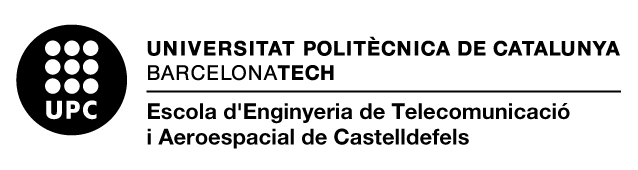
\includegraphics[width=0.5\textwidth]{./setup/EETAC-positiu-negre}
\caption{Exemple de figura}
\label{F:prova}
\end{center}
\end{figure}
\end{verbatim}

donant com a resultat la figura \ref{F:prova}.

\begin{figure}[htb]
\begin{center}
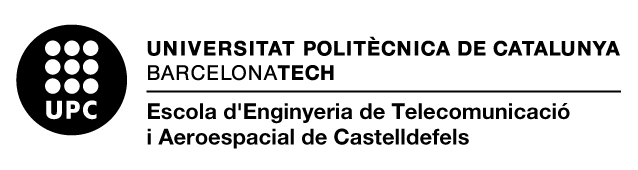
\includegraphics[width=0.5\textwidth]{./setup/EETAC-positiu-negre}
\caption{Exemple de figura}
\label{F:prova}
\end{center}
\end{figure}

Podem tocar la variable \texttt{width} per ajustar l'amplada de la figura com més ens convingui. Teniu en compte que la variable \texttt{textwidth} guarda el valor de l'amplada del texte dins la pàgina i per tant és una bona referència per delimitar amplades de figura, així doncs, la figura \ref{F:prova} ocupa la meitat de l'amplada del texte en una pàgina. 

Podeu arranjar múltiples imatges en una sola figura amb el paquet \texttt{subfigmat}, que defineix un nou entorn \texttt{subfigmatrix} que accepta per argument el nombre de columnes del arranjament. Per exemple, per fer una figura amb tres columnes d'imatges:

\begin{verbatim}
\begin{figure}[htb]
  \begin{center}
    \begin{subfigmatrix}{3}
      \subfigure[Títol subfigura 1]
         {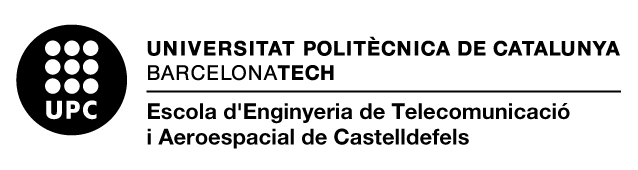
\includegraphics{./setup/EETAC-positiu-negre}\label{SF:S1}} 
      \subfigure[Títol subfigura 2]
         {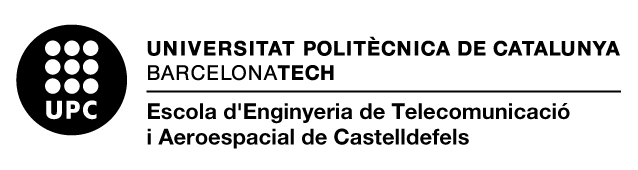
\includegraphics{./setup/EETAC-positiu-negre}\label{SF:S2}} 
      \subfigure[Títol subfigura 3]
         {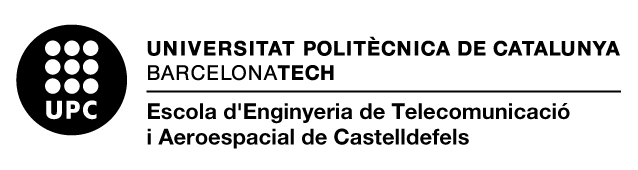
\includegraphics{./setup/EETAC-positiu-negre}\label{SF:S3}} 
      \subfigure[Títol subfigura 4]
         {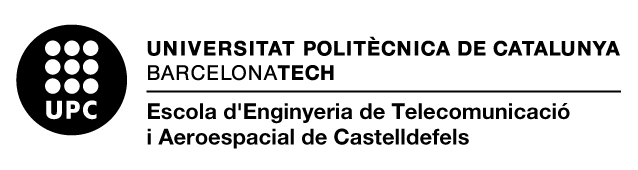
\includegraphics{./setup/EETAC-positiu-negre}\label{SF:S4}} 
      \subfigure[Títol subfigura 5]
         {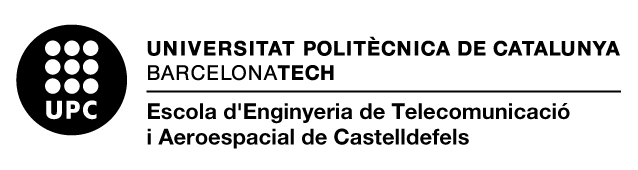
\includegraphics{./setup/EETAC-positiu-negre}\label{SF:S5}} 
      \subfigure[Títol subfigura 6]
         {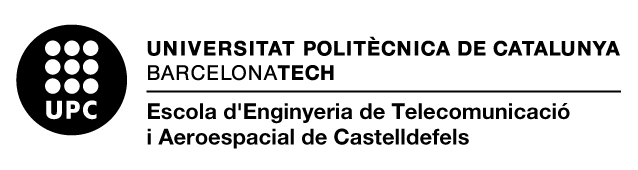
\includegraphics{./setup/EETAC-positiu-negre}\label{SF:S6}} 
    \end{subfigmatrix}
    \caption{Exemple d'arranjament amb múltiples imatges}
    \label{F:prova2}
  \end{center}
\end{figure}
\end{verbatim}

que dona com a resultat, la figura \ref{F:prova2}.

\begin{figure}[htb]
  \begin{center}
    \begin{subfigmatrix}{3}
      \subfigure[Títol subfigura 1]{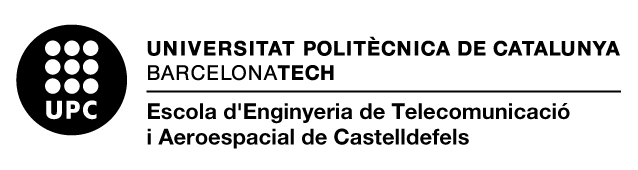
\includegraphics{./setup/EETAC-positiu-negre}\label{SF:S1}} 
      \subfigure[Títol subfigura 2]{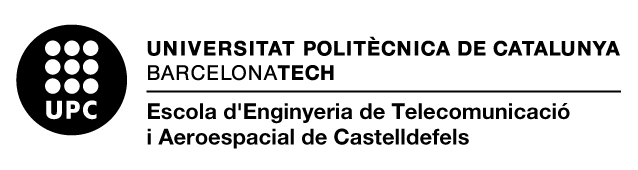
\includegraphics{./setup/EETAC-positiu-negre}\label{SF:S2}} 
      \subfigure[Títol subfigura 3]{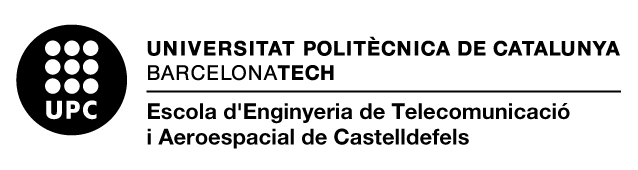
\includegraphics{./setup/EETAC-positiu-negre}\label{SF:S3}} 
      \subfigure[Títol subfigura 4]{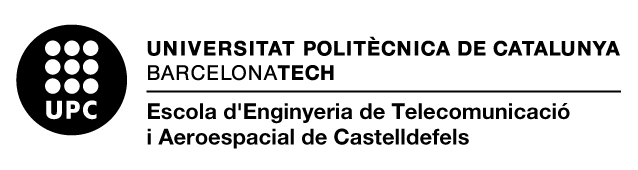
\includegraphics{./setup/EETAC-positiu-negre}\label{SF:S4}} 
      \subfigure[Títol subfigura 5]{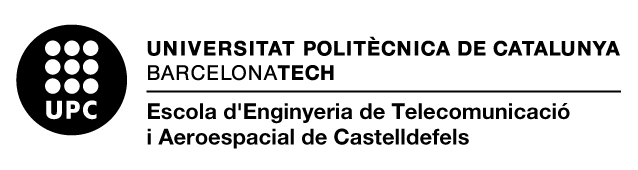
\includegraphics{./setup/EETAC-positiu-negre}\label{SF:S5}} 
      \subfigure[Títol subfigura 6]{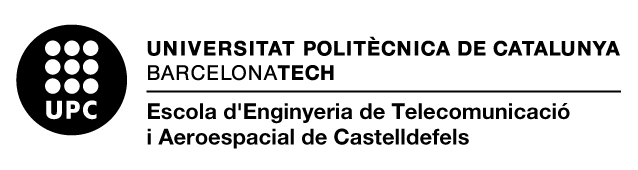
\includegraphics{./setup/EETAC-positiu-negre}\label{SF:S6}} 
    \end{subfigmatrix}
    \caption{Exemple d'arranjament amb múltiples imatges}
    \label{F:prova2}
  \end{center}
\end{figure}

%%%%%%%%%%%%%%%%%%%%%%%%%%%%%%%%%%%%%%%%%%%%%%%%%%%%%%%%%%%%%%%%%%%%%%%%%%%%%%


\subsubsection{Taules}

Pel que fa a la numeració de les taules, no cal fer gran cosa. \LaTeX \ ja fa gran part de la feina bruta. 

Simplement el que heu de fer és inserir la figura amb el codi següent:

\begin{verbatim}
\begin{table}[htb]
\begin{center}
\begin{tabular}{|c|l|r|}
\hline
{\bf Títol de la Columna 1} & {\bf Títol de la Columna 2} & 
{\bf Títol de la Columna 3}  \\ \hline \hline
centrada        & a l'esquerra    & a la dreta       \\ \hline
centrada        & a l'esquerra    & a la dreta       \\ \hline
centrada        & a l'esquerra    & a la dreta       \\ \hline
centrada        & a l'esquerra    & a la dreta       \\ \hline
centrada        & a l'esquerra    & a la dreta       \\ \hline
\end{tabular}
\caption{Exemple de taula}
\label{T:prova}
\end{center}
\end{table}
\end{verbatim}

donant com a resultat la taula \ref{T:prova}.


\begin{table}[htb]
\caption{Exemple de taula}
\begin{center}
\begin{tabular}{|c|l|r|}
\hline
{\bf Títol de la Columna 1} & {\bf Títol de la Columna 2} & {\bf Títol de la Columna 3}  \\ \hline \hline
centrada        & a l'esquerra    & a la dreta       \\ \hline
centrada        & a l'esquerra    & a la dreta       \\ \hline
centrada        & a l'esquerra    & a la dreta       \\ \hline
centrada        & a l'esquerra    & a la dreta       \\ \hline
centrada        & a l'esquerra    & a la dreta       \\ \hline
\end{tabular}
\label{T:prova}
\end{center}
\end{table}

L'entorn \texttt{tabular} que ofereix \LaTeX \ és molt complet i permet crear multitud de taules diferents, tot i que és alhora bastant complexe. Cau fora de les intencions del present document descriure la sintaxis i el format d'aquest tipus d'entorn. És molt fàcil trobar informació al respecte amb llibres especialitzats o simplement a Internet. 


\subsection{Estudi d'ambientalització}

En general l'estudi d'ambientalització es podrà incloure dins de la introducció o a les conclusions, llevat del cas que les repercussions ambientals del treball tinguin una importància tant rellevant que sigui recomanable dedicar-hi un capítol específic.


\subsection{Bibliografia}

Tret que el treball consisteixi en la cerca de bibliografia sobre un tema concret, la bibliografia ha de contenir només la llista d'obres consultades.

A la bibliografia s'han de llistar conjuntament llibres i articles de revistes. Citar una referència bibliogràfica és tant fàcil com fer:

\begin{verbatim}
\cite{prova1}
\end{verbatim}

per citar la referència \cite{prova1}.

El format de la bibliografia es genera automàticament. Un altre (gran!) avantatge del \LaTeX \ :-)


\section{Apèndixs}

En general, cal posar als apèndixs totes les dades i documents que farien el text feixuc i dificultarien la seva lectura, sense oblidar que les contínues referències als apèndixs poden obligar al lector a interrompre constantment la lectura del treball. És per això, que els apèndixs poden incloure diagrames, dades estadístiques, taules de resultats i desenvolupaments teòrics complementaris.

En el cas que, amb el conjunt d'apèndixs, el treball tingui una extensió superior als 100 fulls (aproximadament 200 pàgines), els apèndixs s'han de enquadernar en un volum separat del cos principal del treball. Aquesta plantilla ja proporciona les eines necessàries per fer la portada necessària en cas d'enquadernar els apèndixs per separat.

\cleardoublepage
\phantomsection
\chapter*{Conclusions}

\colorbox{yellow}{TODO}



%%%  BIBLIOGRAFIA
%%%%%%%%%%%%%%%%%%%%%%%%%%%%%%%%%%%%%%%%%%%%%%%%%%%%%%%%%%%%%%%%%%%%%%%%%%

%%% Per la bibliografia hi ha 2 opcions: generarla amb la utilitat BibTeX 
%%%                                      o fer-la ''a ma''
%%% NOTA: podeu trobar facilment informació sobre BibTeX a:
%%%  http://www.ctan.org/tex-archive/biblio/bibtex/contrib/doc/

%%% OPCIO 1: BibTeX (recomanat) -> descomentar les comandes seguents:
%\bibliographystyle{unsrt}   %% Estil de bibliografia EETAC
%\cleardoublepage
%\phantomsection
% Indicar aqui el(s) fitxer(s) que contenen la bibliografia
%\bibliography{fitxer1,...,fitxerN}  
%\pdfbookmark{Bibliografia}{sec:biblio}

%%% OPCIO 2: bibliografia manual
%%%
%%% L'argument d'entrada es el numero de referencies que s'inclouen
\cleardoublepage
\phantomsection
\begin{thebibliography}{2}

%% Llibres:  Autor/s (cognoms i inicials dels noms), títol del llibre (en cursiva), editor, ciutat i any de publicació. Quan es cita el capítol d'un llibre s'ha d'indicar el títol del capítol (entre cometes), el títol del llibre (en cursiva) i els números de pàgines amb la primera i la darrera incloses.

%%  Exemple de capitol en llibre
\bibitem{prova1} 
Cognoms-autor, Inicial-nom.
``Títol del capítol''. {\it Títol del llibre}.
(Editor. Ciutat. Any publicació): pagina1--paginaN.

%%  Exemple de d'article en revista
\bibitem{prova2} 
Cognoms-autor, Inicial-nom.
``Títol de l'article''. {\it Títol de la revista}.
{\bf volum}(numero),
pagina1--paginaN. (Any publicació) 

\end{thebibliography}

%%%%%%%%%%%%%%%%%%%%%%%%%%%%%%%%%%%%%%%%%%%%%%%%%%%%%%%%%%%%%%%%%%%%%%%%%%
%%%%%%                           APENDIXS                         %%%%%%%%
%%%%%%%%%%%%%%%%%%%%%%%%%%%%%%%%%%%%%%%%%%%%%%%%%%%%%%%%%%%%%%%%%%%%%%%%%%
\pagestyle{empty}  % no tocar

%% Descomentar una de les dues línies següents, en funció de:
%%  a) els apendixs s'encuadernaran apart (amb portada) 
%%  b) els apendixs s'enquadernen amb el mateix projecte (sense portada). 
%% Recordeu que si tot el document (amb apèndixs) excedeix les 100 pagines 
%% s'ha d'enquadernar a part
%\appendix\ambportada
\appendix\senseportada


%%%%%%%%%%%%%%%%%%%%%%%%%%%%%%%%%%%%%%%%%%%%%%%%%%%%%%%%%%%%%%%%%%%%%%%%%%
%%%%%% INCLOURE A PARTIR D'AQUI TOTS ELS CAPÍTOLS DELS APENDIXS   %%%%%%%%
%%%%%%%%%%%%%%%%%%%%%%%%%%%%%%%%%%%%%%%%%%%%%%%%%%%%%%%%%%%%%%%%%%%%%%%%%%

\chapter{Exemple de prova d'un apèndix}

Text de prova



%%%%%%%%%%%%%%%%%%%%%%%%%%%%%%%%%%%%%%%%%%%%%%%%%%%%%%%%%%%%%%%%%%%%%%%%%%
%%%%%%%%%%%%%%%%%%%%%%%%%%%%%%%%%%%%%%%%%%%%%%%%%%%%%%%%%%%%%%%%%%%%%%%%%%
%%%%%%%%%%%%%%%%%%%%%%%%%%%%%%%%%%%%%%%%%%%%%%%%%%%%%%%%%%%%%%%%%%%%%%%%%%
% i  aixo es tot! ;)
\end{document}






